\documentclass{jsarticle}
\usepackage[dvipdfmx]{graphics}
\usepackage{amsmath}
\usepackage{amssymb}
\usepackage{ascmac}
\usepackage{bm}
\usepackage{url}
\usepackage{txfonts}

\newcommand{\mmm}{\hspace{3mm}}
\newcommand{\veczero}{$\vec{0}$}
\newcommand{\veca}{$\vec{a}$}
\newcommand{\vecb}{$\vec{b}$}
\newcommand{\veco}{$\vec{o}$}
\newcommand{\vecx}{$\vec{x}$}
\newcommand{\vecy}{$\vec{y}$}
\newcommand{\vecz}{$\vec{z}$}
\newcommand{\mathins}[1]{${#1}$}


\begin{document}
    \section{(1,2)のようなベクトル}
    これは見るからに数字のみの形式をしている.このような表記のベクトルは予めお約束となるベクトルを用意することで向きの計算を回避している.
    \subsection{(1,2)の意味}
    (1,2)のような形をしているベクトルは次のようにあらわすこともできる.
    \[
    (1,2)=\vec{x}+2\vec{y}
    \]
    ここでの$\vec{x}$とはx軸正方向に大きさ1のベクトルを表し,$\vec{y}$はy軸正方向に大きさ1のベクトルを表している.大きさ1のベクトルを特別に単位ベクトルという.この各軸の正方向に向く単位ベクトルをお約束のベクトルとして用意し,その係数だけでベクトルを表すのが(1,2)のようなベクトルの意味だ.

    \subsection{計算}

    前の節の話を持ってくれば$\vec{x},\vec{y}$があれば,あとは係数の計算をするだけで足し算と引き算は計算できる.
    \begin{eqnarray*}
        &&(1,2)+(3,-7)=(1+3,2-7)=(4,-5)\\
        &&(\vec{x}+2\vec{y})+(3\vec{x}-7\vec{y})=4\vec{x}-5\vec{y}
    \end{eqnarray*}

    次は定数倍だ.
    \begin{eqnarray*}
        &&k(1,2)=(k,2k)\\
        &&k(\vec{x}+2\vec{y}) =k\vec{x}+2k\vec{y}
    \end{eqnarray*}
    各成分に定数をかければいい.


    最後は内積だ.だが,その前にお約束のベクトルのみで内積などを計算しておく.
    \[
    \vec{x}\cdot\vec{x}=1,\mmm\vec{y}\cdot\vec{y}=1,\mmm\vec{x}\cdot\vec{y}=0
    \]
    大きさ1であることと,軸は直交していることから計算される.

    これを使って次の内積を計算する\footnote{$(a,b)\cdot(c,d)$という書き方は誤りです.答案には書かないようにしましょう.}.
    \begin{eqnarray*}
        \vec{n}=(a,b),&\mmm&\vec{m}=(c,d)\\
        \vec{n}\cdot\vec{m}&=&(a\vec{x}+b\vec{y})(c\vec{x}+d\vec{y})\\
        &=&ac|\vec{x}|^2 +(ad+bc)\vec{x}\cdot\vec{y}+bd|\vec{y}|^2\\
        &=&ac+bd
    \end{eqnarray*}
    x成分同士,y成分同士の積を足せばよいことがわかる.

    また,複数のベクトルの和としてあらわされているベクトルを掛け算(内積)するときは前もって部分的な内積,大きさの2乗を示す形の書き方をするほうが答案として簡潔でよい.

    \subsection{使用の方針}
    ベクトル入門の章において係数のみによってベクトルを表すタイプを前面に使うことはない.例えば(1,2),(3,4)が与えられていたら,$\vec{a}=(1,2),\vec{b}=(3,4)$として\veca ,\vecb によって計算を進める.そして計算が一段落したら$|\vec{a}|^2=1^2+2^2,|\vec{b}|^2=3^2+4^2,\vec{a}\cdot\vec{b}=3+2\times4$を使う.

    ベクトル入門の章における計算の位置づけは次の図\ref{fig:vector_sanjutukeisan_taikei}のようになっている.

    \begin{figure}[htbp]
        \begin{center}
            \resizebox{!}{6cm}{
            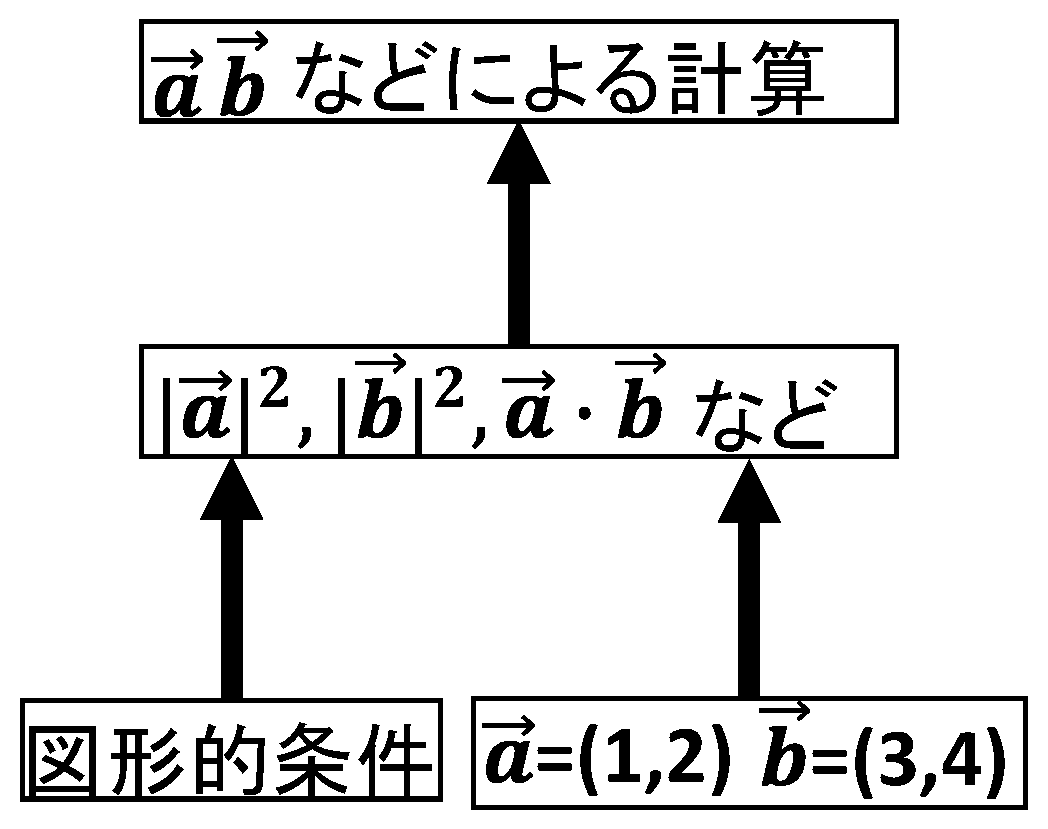
\includegraphics{img/vector_sanjutukeisan_taikei.eps}
            }
        \end{center}
        \caption{ベクトル計算の体系}
        \label{fig:vector_sanjutukeisan_taikei}
    \end{figure}

    したがって,ベクトル入門の章において成分表示で与えられたベクトルは問題の条件と同等の扱いをする.

    \section{ベクトル入門での問題}
    この章の内容で理解できる問題は以下の通りだ.
    \begin{itemize}
        \item 2ベクトルの関係(垂直)
        \item 2ベクトルの関係(平行)
        \item 2ベクトルの関係(角度)
        \item 2点間の距離
        \item ベクトルの成分分解
        \item ベクトルの分解
    \end{itemize}

    以下に問題を示す.解く必要はないので解答を読んでほしい.

    \subsection{2ベクトルの関係(垂直)}
    \begin{itembox}[l]{問題}
        \begin{enumerate}
            \item $\vec{a}=(1,2)$と垂直であり,なおかつ大きさが$2\sqrt{5}$のベクトルを答えよ.
            \item $\vec{b}=(3,0,0)$と垂直なベクトルを2つ挙げよ.ただし,その2つのベクトル同士も垂直であるとする.
        \end{enumerate}
    \end{itembox}

    まずは1番の問題からだ.未知のベクトルを$\vec{x}=(a,b)$とおいて
    \[
    \left\{
    \begin{array}{c}
        a+2b=0\\
        a^2+b^2=20
    \end{array}
    \right.
    \]
    を解けば答えが$(-4,2),(4,-2)$と出る.しかし,これでは芸がない.勘が良いのであれば(1,2)の位置を入れ替え(2,1)とし,どちらかを-1倍することで元のベクトルと垂直なベクトルが得られることがわかるだろう.そうすると,-1倍するのはx成分か,y成分なのかで答えが2つとなることも合点がいく.これを図\ref{fig:vector_90_kaiten}に表してみよう.
    %
    \begin{figure}[htbp]
        \begin{center}
            \resizebox{!}{4cm}{
            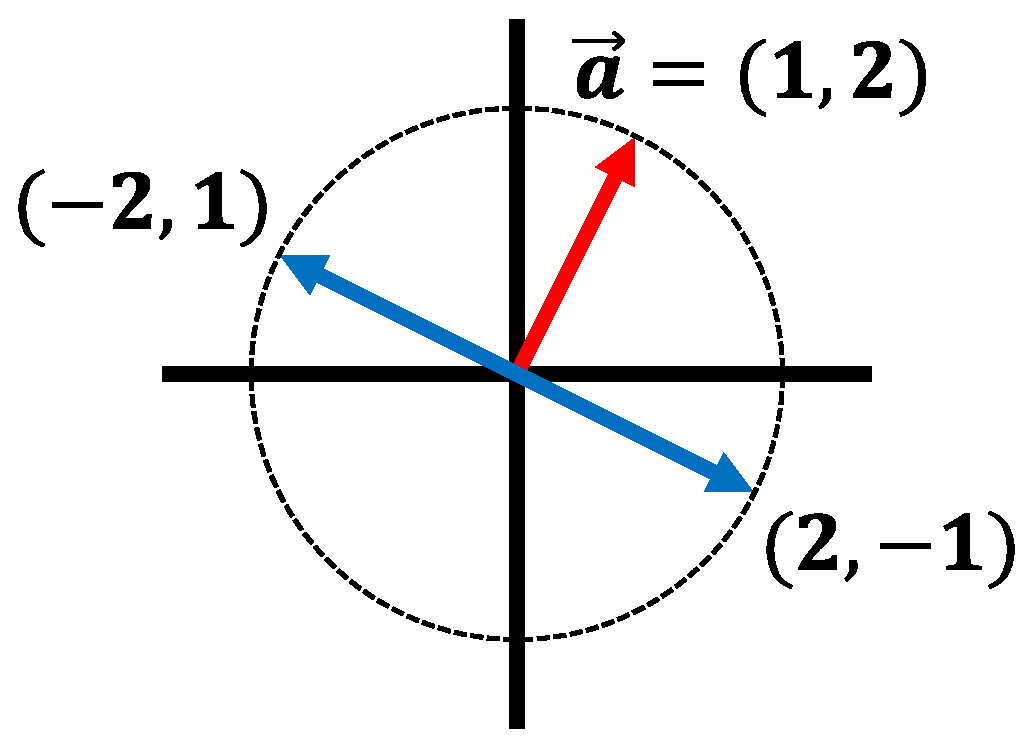
\includegraphics{img/vector_90_kaiten.eps}
            }
        \end{center}
        \caption{ベクトルの回転}
        \label{fig:vector_90_kaiten}
    \end{figure}

    このようにx成分を-1倍すると正の方向に$90^\circ$,y成分を-1倍すると負の方向に$90^\circ$回転することがわかる.これをベクトルの回転\footnote{ベクトルの回転は後の章で扱う.}という.

    回転の発想は法線を扱うときに有効なので頭の隅に置いておきたい.

    2番の問題は3次元ベクトルだ.3つ目の成分はz軸に正方向な単位ベクトルの係数を表している.これは3次元ベクトルの導入に過ぎず,答えの例は(0,1,0),(0,0,1)が挙げられる.3次元ベクトルは計算量こそ多いが2次元ベクトルと同じ話が通用するので拒否反応を起こさないでほしい.

    \subsection{2ベクトルの関係(平行)}
    \begin{itembox}[l]{問題}
        \begin{enumerate}
            \item $\vec{a}=(3,4)$と平行であり,なおかつ大きさが$10$のベクトルを答えよ.
            \item $\vec{b}=(2,5,7)$と平行であり,なおかつ大きさが$19$のベクトルを答えよ.
            \item 四角形ABCDにおいて$\overrightarrow{\mathrm{AB}}=\overrightarrow{\mathrm{DC}}$であるとき,四角形ABCDはどのような四角形であると考えられるか.すべて答えよ.
        \end{enumerate}
    \end{itembox}

    1番の問題は未知のベクトルを$k(3,4)$と置いて次の方程式を解けばよい.
    \[
    25k^2=10^2
    \]
    これより$k=\pm 2$となるので答えは(6,8),(-6,-8)の2つとなる.

    次に2番目の問題だが,これも実数$k$を用意して未知のベクトルを$k(2,5,7)$と置いて計算するのもよいが,この問いではそれが面倒なようにしてある.ここでは単位ベクトルを計算することで答えを求めたい.単位ベクトルは何らかのベクトルを,その大きさで割ることで計算できる.つまり(2,5,7)と同じ向きの単位ベクトルは
    \[
    \frac{1}{\sqrt{2^2+5^2+7^2}}(2,5,7)=\frac{1}{\sqrt{78}}(2,5,7)
    \]
    あとは,大きさが19となるようにすればいいので,答えは
    \[
    \frac{19}{\sqrt{78}}(2,5,7),\mmm \frac{-19}{\sqrt{78}}(2,5,7)
    \]
    の2つとなる.平行なベクトルの計算は単位ベクトルを経由したほうが簡単なことがあるので,発想の引き出しにあるとうれしい.

    最後の問題はベクトルによって平面図形を考える入り口となるような問題だ.問題文より$\overrightarrow{\mathrm{AB}}=\overrightarrow{\mathrm{DC}}$であるがこれは線分$AB$と線分$DC$が大きさが等しく,なおかつ平行であることを示している.これは1組の辺が等しく平行だという平行四辺形の条件を示している.ここから答えは平行四辺形または,ひし形であるとわかる.

    \subsection{2ベクトルの関係(角度)}
    \begin{itembox}[l]{問題}
        \begin{enumerate}
            \item $\vec{a}=(\sqrt{3},1),\vec{b}=(0,2)$のなす角を求めよ.
            \item $\vec{c}=(1,\sqrt{3}),\vec{d}=(t,1)$としたとき,$\vec{c},\vec{d}$が垂直となるときの$t$の値を求めよ.またこのとき,$\vec{d}$がx軸正方向となす角を求めよ.
        \end{enumerate}
    \end{itembox}
    1番の問題は内積の式を変形することで$\cos\theta$を計算することで求められる.\veczero ではない2つのベクトル\veca ,\vecb に対しては次の式が成立する.
    \[
    \cos\theta =\frac{\vec{a}\cdot\vec{b}}{|\vec{a}||\vec{b}|}
    \]
    あとは今回の問題の条件より$\vec{a}\cdot\vec{b}=2,|\vec{a}|=2,|\vec{b}|=2$なので
    \[
    \cos\theta =\frac{1}{2}\mmm \Rightarrow \mmm \theta=60^\circ
    \]

    2番の問題は内積が0という直角の条件から容易に計算できる.
    \[
    t+\sqrt{3}=0\mmm \therefore t=-\sqrt{3}
    \]
    ここから
    \[
    \vec{d}=(-\sqrt{3},1)
    \]
    とわかる.x軸とのなす角は$\tan\theta$を考えるのがよく,求める角度を$\varphi$とすると
    \[
    \tan\varphi = -\frac{1}{\sqrt{3}}\mmm\Rightarrow\mmm\varphi = 150^\circ
    \]
    となる.

    \subsection{2点間の距離}
    \begin{itembox}[l]{問題}
        始点を共有する2つのベクトル\veca ,\vecb は$|\vec{a}|=2,|\vec{b}|=3$,なす角は$\theta=60^\circ$である.このとき2つのベクトルの先端をつないだ線分の長さを求めよ.

        また,この導出にあたり現れる定理は何か.
        %
    \end{itembox}

    ベクトルの先端の長さを考えるとは$|\vec{a}-\vec{b}|$の計算と分かれば話は早い.まずは条件より$\vec{a}\cdot\vec{b}=3$と計算する.あとは大きさの2乗を計算する.
    \begin{eqnarray*}
        |\vec{a}-\vec{b}|^2 &=& |\vec{a}|^2+|\vec{b}|^2-2\vec{a}\cdot\vec{b}\\
        &=&4+9-6=7\\
        \therefore |\vec{a}-\vec{b}|&=&\sqrt{7}
    \end{eqnarray*}

    \begin{figure}[htbp]
    \begin{center}
        \resizebox{!}{3cm}{
        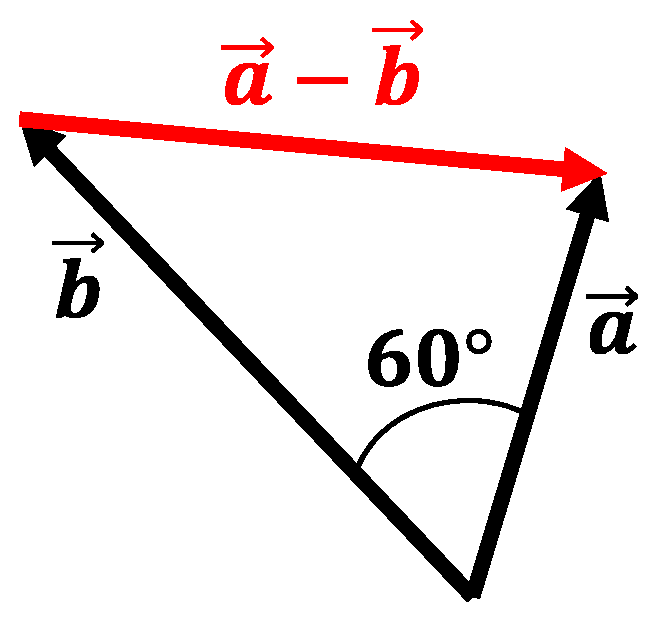
\includegraphics{img/vector_nyumon1.eps}
        }
    \end{center}
    \caption{2点間の距離}
    \label{fig:vector_nyumon1}
    \end{figure}
    ベクトルとスカラを結ぶ方法のおさらいとなる問題だ.そしてこの問題の式を図\ref{fig:vector_nyumon1}とともに見てみる.
    \[
    |\vec{a}-\vec{b}|^2 = |\vec{a}|^2+|\vec{b}|^2-2\vec{a}\cdot\vec{b}
    \]
    をベクトルではない表記に変えてみる.
    \[
    \mathrm{AB}^2 =\mathrm{OA}^2+\mathrm{OB}^2-2 \mathrm{OA}\cdot \mathrm{OB}\cos\theta
    \]
    これは紛れもない余弦定理の公式だ.これはベクトルを利用した余弦定理の証明となっている.


    \subsection{ベクトルの成分分解}
    ベクトルと座標を結びつけるために必要な知識だ.
    \begin{itembox}[l]{問題}
        \begin{enumerate}
            \item 大きさ2,x軸の正方向となす角が$30^\circ$のベクトルのx成分とy成分を答えよ.
            \item 大きさ1,x軸の正方向となす角が$\alpha$となるベクトルを\veca ,大きさ1,x軸の正方向となす角が$\beta$となるベクトルを\vecb とする.$\vec{a}+\vec{b}$のx成分とy成分を2通りの方法で表現せよ.
        \end{enumerate}
    \end{itembox}

    1番の問題は数3における極座標の理解に共通する.答えは$(2\cos30^\circ,2\sin30^\circ)=(1,\sqrt{3})$となる.
    %

    次の問題こそ図がないとわからないだろう.問題の性質上$\alpha<\beta$として問題ない\footnote{2つの単位ベクトルのうち,x軸の正方向となす角が小さいほうを$\alpha$,大きいほうを$\beta$としているに過ぎない.}.
    %
    \begin{figure}[htbp]
        \begin{center}
            \resizebox{!}{5cm}{
            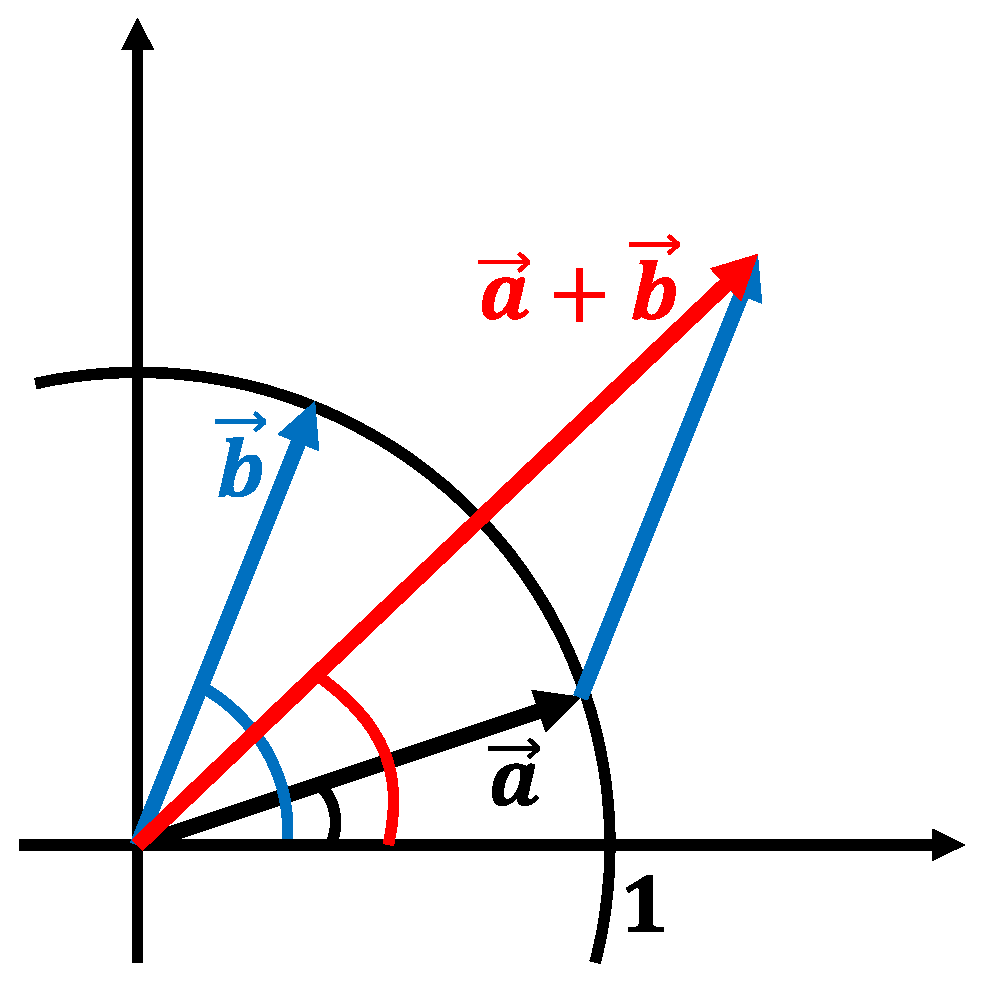
\includegraphics{img/vector_nyumon2.eps}
            }
        \end{center}
        \caption{単位ベクトルの和}
        \label{fig:vector_nyumon2}
    \end{figure}
    まずは1通り目の表現だ.これは単純に成分ごとの計算をすればいい.
    \[
    \vec{a}+\vec{b}=(\cos\alpha+\cos\beta,\mmm\sin\alpha+\sin\beta)
    \]
    次は図\ref{fig:vector_nyumon2}を見てそこから成分表示をする.角度は$\alpha,\beta$の平均をとればいい.あとは$|\vec{a}+\vec{b}|$がわかればいい.これはすでに解いた問題と同じだ.
    \begin{eqnarray*}
        |\vec{a}+\vec{b}|^2&=& |\vec{a}|^2+|\vec{b}|^2 +2\vec{a}\cdot\vec{b}\\
        &=& 2+2\cos(\beta-\alpha)\\
        &=& 2 +2\left(2\cos^2\frac{\beta-\alpha}{2}-1\right)\mmm
        \left(\because \cos\theta=2\cos^2\frac{\theta}{2}-1\right)\\
        &=&4\cos^2\frac{\beta-\alpha}{2}
    \end{eqnarray*}
    さて$\beta-\alpha$はベクトルのなす角であるから$0<|\beta-\alpha|<\pi$である.その半分は$0<|(\beta-\alpha)/2|<\pi/2$と分かる.ここから
    \[
    \cos\frac{\beta-\alpha}{2}=\cos\frac{\alpha-\beta}{2}>0
    \]
    となる.
    \[
    |\vec{a}+\vec{b}|^2=4\cos^2\frac{\beta-\alpha}{2}\mmm \Rightarrow\mmm
    |\vec{a}+\vec{b}|=2\cos\frac{\alpha-\beta}{2}
    \]
    最終的に2つ目の成分表示は
    \[
    \vec{a}+\vec{b}= \left(
    2\cos\frac{\alpha-\beta}{2}\cos\frac{\alpha+\beta}{2},\mmm2\cos\frac{\alpha-\beta}{2}\sin\frac{\alpha+\beta}{2}
    \right)
    \]
    となる.

    問題自体はこれで終わりだが,2番の問題の結果からx,yの成分同士で等式を立てることで次の2式を得ることができる.
    \begin{eqnarray*}
        \cos\alpha+\cos\beta &=&2\cos\frac{\alpha-\beta}{2}\cos\frac{\alpha+\beta}{2}\\
        \sin\alpha+\sin\beta &=&2\cos\frac{\alpha-\beta}{2}\sin\frac{\alpha+\beta}{2}
    \end{eqnarray*}
    これは三角関数の和積の公式だ.ベクトルを用いて三角関数の公式の導出をしたことになる.

    \subsection{ベクトルの分解}
    ベクトルを任意の2つのベクトルの和に分解するという問題だ.これは単に連立方程式の問題となるが色々なところに現れる発想だ.
    \begin{itembox}[l]{問題}
        \begin{enumerate}
            \item ベクトル(1,2)を$\vec{a}=(3,-4),\vec{b}=(-5,7)$を用いた式で表せ.
            \item ベクトル(1,-1)を\mathins{\vec{a}=(3,4),\vec{b}=(4,-3)}を用いた式で表せ.ただし,\mathins{\vec{a}\cdot\vec{b}=0}であることを用いること.
        \end{enumerate}
    \end{itembox}
    1番の問題は\veca ,\vecb の係数を$x,y$とすると
    \[
    (1,2)=x(3,-4)+y(-5,7)
    \]
    という式が立つ.あとは成分ごとに分けて連立方程式とすると$x=17,y=10$を得る.単純な問題である.

    2番の解法が発想として少しだけ大事である.こちらも1番と同様にして連立方程式を立てれば計算はできる.しかし,これでは内積の利用ができない.\mathins{\vec{f}=(1,-1)}として以下のように計算される.
    \begin{align*}
        \vec{f} &= x\vec{a}+y\vec{b}\\
        \vec{f}\cdot\vec{a}&= x\vec{a}\cdot\vec{a} +y\vec{b}\cdot\vec{a}\\
        &= x |\vec{a}|^2 \quad (\because \vec{a}\perp \vec{b})\\
        \therefore x &= \frac{\vec{f}\cdot\vec{a}}{|\vec{a}|^2}\\\\
        \vec{f}\cdot\vec{b}&= x\vec{a}\cdot\vec{b} +y\vec{b}\cdot\vec{b}\\
        &= y|\vec{b}|^2 \quad (\because \vec{a}\perp \vec{b})\\
        \therefore y&=\frac{\vec{f}\cdot\vec{b}}{|\vec{b}|^2}
    \end{align*}

    計算すると\mathins{x=\frac{-1}{25},y=\frac{7}{25}}となる.
    垂直であるという条件はベクトルを扱う上で最も強力な条件の1つである.その恩恵は計り知れないので常にベクトルのなす角には注意が必要だ.




\end{document}
